% Options for packages loaded elsewhere
\PassOptionsToPackage{unicode}{hyperref}
\PassOptionsToPackage{hyphens}{url}
\PassOptionsToPackage{dvipsnames,svgnames,x11names}{xcolor}
%
\documentclass[
  letterpaper,
  DIV=11,
  numbers=noendperiod]{scrartcl}

\usepackage{amsmath,amssymb}
\usepackage{lmodern}
\usepackage{iftex}
\ifPDFTeX
  \usepackage[T1]{fontenc}
  \usepackage[utf8]{inputenc}
  \usepackage{textcomp} % provide euro and other symbols
\else % if luatex or xetex
  \usepackage{unicode-math}
  \defaultfontfeatures{Scale=MatchLowercase}
  \defaultfontfeatures[\rmfamily]{Ligatures=TeX,Scale=1}
\fi
% Use upquote if available, for straight quotes in verbatim environments
\IfFileExists{upquote.sty}{\usepackage{upquote}}{}
\IfFileExists{microtype.sty}{% use microtype if available
  \usepackage[]{microtype}
  \UseMicrotypeSet[protrusion]{basicmath} % disable protrusion for tt fonts
}{}
\makeatletter
\@ifundefined{KOMAClassName}{% if non-KOMA class
  \IfFileExists{parskip.sty}{%
    \usepackage{parskip}
  }{% else
    \setlength{\parindent}{0pt}
    \setlength{\parskip}{6pt plus 2pt minus 1pt}}
}{% if KOMA class
  \KOMAoptions{parskip=half}}
\makeatother
\usepackage{xcolor}
\usepackage[top=1in,left=1in,right=1in,bottom=1in]{geometry}
\setlength{\emergencystretch}{3em} % prevent overfull lines
\setcounter{secnumdepth}{-\maxdimen} % remove section numbering
% Make \paragraph and \subparagraph free-standing
\ifx\paragraph\undefined\else
  \let\oldparagraph\paragraph
  \renewcommand{\paragraph}[1]{\oldparagraph{#1}\mbox{}}
\fi
\ifx\subparagraph\undefined\else
  \let\oldsubparagraph\subparagraph
  \renewcommand{\subparagraph}[1]{\oldsubparagraph{#1}\mbox{}}
\fi

\usepackage{color}
\usepackage{fancyvrb}
\newcommand{\VerbBar}{|}
\newcommand{\VERB}{\Verb[commandchars=\\\{\}]}
\DefineVerbatimEnvironment{Highlighting}{Verbatim}{commandchars=\\\{\}}
% Add ',fontsize=\small' for more characters per line
\usepackage{framed}
\definecolor{shadecolor}{RGB}{241,243,245}
\newenvironment{Shaded}{\begin{snugshade}}{\end{snugshade}}
\newcommand{\AlertTok}[1]{\textcolor[rgb]{0.68,0.00,0.00}{#1}}
\newcommand{\AnnotationTok}[1]{\textcolor[rgb]{0.37,0.37,0.37}{#1}}
\newcommand{\AttributeTok}[1]{\textcolor[rgb]{0.40,0.45,0.13}{#1}}
\newcommand{\BaseNTok}[1]{\textcolor[rgb]{0.68,0.00,0.00}{#1}}
\newcommand{\BuiltInTok}[1]{\textcolor[rgb]{0.00,0.23,0.31}{#1}}
\newcommand{\CharTok}[1]{\textcolor[rgb]{0.13,0.47,0.30}{#1}}
\newcommand{\CommentTok}[1]{\textcolor[rgb]{0.37,0.37,0.37}{#1}}
\newcommand{\CommentVarTok}[1]{\textcolor[rgb]{0.37,0.37,0.37}{\textit{#1}}}
\newcommand{\ConstantTok}[1]{\textcolor[rgb]{0.56,0.35,0.01}{#1}}
\newcommand{\ControlFlowTok}[1]{\textcolor[rgb]{0.00,0.23,0.31}{#1}}
\newcommand{\DataTypeTok}[1]{\textcolor[rgb]{0.68,0.00,0.00}{#1}}
\newcommand{\DecValTok}[1]{\textcolor[rgb]{0.68,0.00,0.00}{#1}}
\newcommand{\DocumentationTok}[1]{\textcolor[rgb]{0.37,0.37,0.37}{\textit{#1}}}
\newcommand{\ErrorTok}[1]{\textcolor[rgb]{0.68,0.00,0.00}{#1}}
\newcommand{\ExtensionTok}[1]{\textcolor[rgb]{0.00,0.23,0.31}{#1}}
\newcommand{\FloatTok}[1]{\textcolor[rgb]{0.68,0.00,0.00}{#1}}
\newcommand{\FunctionTok}[1]{\textcolor[rgb]{0.28,0.35,0.67}{#1}}
\newcommand{\ImportTok}[1]{\textcolor[rgb]{0.00,0.46,0.62}{#1}}
\newcommand{\InformationTok}[1]{\textcolor[rgb]{0.37,0.37,0.37}{#1}}
\newcommand{\KeywordTok}[1]{\textcolor[rgb]{0.00,0.23,0.31}{#1}}
\newcommand{\NormalTok}[1]{\textcolor[rgb]{0.00,0.23,0.31}{#1}}
\newcommand{\OperatorTok}[1]{\textcolor[rgb]{0.37,0.37,0.37}{#1}}
\newcommand{\OtherTok}[1]{\textcolor[rgb]{0.00,0.23,0.31}{#1}}
\newcommand{\PreprocessorTok}[1]{\textcolor[rgb]{0.68,0.00,0.00}{#1}}
\newcommand{\RegionMarkerTok}[1]{\textcolor[rgb]{0.00,0.23,0.31}{#1}}
\newcommand{\SpecialCharTok}[1]{\textcolor[rgb]{0.37,0.37,0.37}{#1}}
\newcommand{\SpecialStringTok}[1]{\textcolor[rgb]{0.13,0.47,0.30}{#1}}
\newcommand{\StringTok}[1]{\textcolor[rgb]{0.13,0.47,0.30}{#1}}
\newcommand{\VariableTok}[1]{\textcolor[rgb]{0.07,0.07,0.07}{#1}}
\newcommand{\VerbatimStringTok}[1]{\textcolor[rgb]{0.13,0.47,0.30}{#1}}
\newcommand{\WarningTok}[1]{\textcolor[rgb]{0.37,0.37,0.37}{\textit{#1}}}

\providecommand{\tightlist}{%
  \setlength{\itemsep}{0pt}\setlength{\parskip}{0pt}}\usepackage{longtable,booktabs,array}
\usepackage{calc} % for calculating minipage widths
% Correct order of tables after \paragraph or \subparagraph
\usepackage{etoolbox}
\makeatletter
\patchcmd\longtable{\par}{\if@noskipsec\mbox{}\fi\par}{}{}
\makeatother
% Allow footnotes in longtable head/foot
\IfFileExists{footnotehyper.sty}{\usepackage{footnotehyper}}{\usepackage{footnote}}
\makesavenoteenv{longtable}
\usepackage{graphicx}
\makeatletter
\def\maxwidth{\ifdim\Gin@nat@width>\linewidth\linewidth\else\Gin@nat@width\fi}
\def\maxheight{\ifdim\Gin@nat@height>\textheight\textheight\else\Gin@nat@height\fi}
\makeatother
% Scale images if necessary, so that they will not overflow the page
% margins by default, and it is still possible to overwrite the defaults
% using explicit options in \includegraphics[width, height, ...]{}
\setkeys{Gin}{width=\maxwidth,height=\maxheight,keepaspectratio}
% Set default figure placement to htbp
\makeatletter
\def\fps@figure{htbp}
\makeatother

\KOMAoption{captions}{tableheading}
\makeatletter
\@ifpackageloaded{tcolorbox}{}{\usepackage[many]{tcolorbox}}
\@ifpackageloaded{fontawesome5}{}{\usepackage{fontawesome5}}
\definecolor{quarto-callout-color}{HTML}{909090}
\definecolor{quarto-callout-note-color}{HTML}{0758E5}
\definecolor{quarto-callout-important-color}{HTML}{CC1914}
\definecolor{quarto-callout-warning-color}{HTML}{EB9113}
\definecolor{quarto-callout-tip-color}{HTML}{00A047}
\definecolor{quarto-callout-caution-color}{HTML}{FC5300}
\definecolor{quarto-callout-color-frame}{HTML}{acacac}
\definecolor{quarto-callout-note-color-frame}{HTML}{4582ec}
\definecolor{quarto-callout-important-color-frame}{HTML}{d9534f}
\definecolor{quarto-callout-warning-color-frame}{HTML}{f0ad4e}
\definecolor{quarto-callout-tip-color-frame}{HTML}{02b875}
\definecolor{quarto-callout-caution-color-frame}{HTML}{fd7e14}
\makeatother
\makeatletter
\makeatother
\makeatletter
\@ifpackageloaded{caption}{}{\usepackage{caption}}
\AtBeginDocument{%
\ifdefined\contentsname
  \renewcommand*\contentsname{Table of contents}
\else
  \newcommand\contentsname{Table of contents}
\fi
\ifdefined\listfigurename
  \renewcommand*\listfigurename{List of Figures}
\else
  \newcommand\listfigurename{List of Figures}
\fi
\ifdefined\listtablename
  \renewcommand*\listtablename{List of Tables}
\else
  \newcommand\listtablename{List of Tables}
\fi
\ifdefined\figurename
  \renewcommand*\figurename{Figure}
\else
  \newcommand\figurename{Figure}
\fi
\ifdefined\tablename
  \renewcommand*\tablename{Table}
\else
  \newcommand\tablename{Table}
\fi
}
\@ifpackageloaded{float}{}{\usepackage{float}}
\floatstyle{ruled}
\@ifundefined{c@chapter}{\newfloat{codelisting}{h}{lop}}{\newfloat{codelisting}{h}{lop}[chapter]}
\floatname{codelisting}{Listing}
\newcommand*\listoflistings{\listof{codelisting}{List of Listings}}
\makeatother
\makeatletter
\@ifpackageloaded{caption}{}{\usepackage{caption}}
\@ifpackageloaded{subcaption}{}{\usepackage{subcaption}}
\makeatother
\makeatletter
\@ifpackageloaded{tcolorbox}{}{\usepackage[many]{tcolorbox}}
\makeatother
\makeatletter
\@ifundefined{shadecolor}{\definecolor{shadecolor}{rgb}{.97, .97, .97}}
\makeatother
\makeatletter
\makeatother
\ifLuaTeX
  \usepackage{selnolig}  % disable illegal ligatures
\fi
\IfFileExists{bookmark.sty}{\usepackage{bookmark}}{\usepackage{hyperref}}
\IfFileExists{xurl.sty}{\usepackage{xurl}}{} % add URL line breaks if available
\urlstyle{same} % disable monospaced font for URLs
\hypersetup{
  pdftitle={Diagnostics and Transformations},
  colorlinks=true,
  linkcolor={blue},
  filecolor={Maroon},
  citecolor={Blue},
  urlcolor={Blue},
  pdfcreator={LaTeX via pandoc}}

\title{Diagnostics and Transformations}
\usepackage{etoolbox}
\makeatletter
\providecommand{\subtitle}[1]{% add subtitle to \maketitle
  \apptocmd{\@title}{\par {\large #1 \par}}{}{}
}
\makeatother
\subtitle{Simple linear regression -- Stat 230}
\author{}
\date{}

\begin{document}
\maketitle
\ifdefined\Shaded\renewenvironment{Shaded}{\begin{tcolorbox}[borderline west={3pt}{0pt}{shadecolor}, breakable, sharp corners, boxrule=0pt, frame hidden, enhanced, interior hidden]}{\end{tcolorbox}}\fi

In this class, you will work with your group to explore the adequacy of
simple linear regression models and how transformations can help remedy
some violations of those assumptions. While you work through this
activity, make sure that all group members are engaged and contribute
ideas, and also follow the code. While the R Manual has some useful R
code for today's activities (especially for review), new code is given
as needed.

\hypertarget{assessing-slr-model-assumptions}{%
\subsection{Assessing SLR model
assumptions}\label{assessing-slr-model-assumptions}}

\textbf{Task 1.} To begin, review the assumptions/conditions necessary
for valid inference from simple linear regression models. List the
necessary assumptions/conditions and give at least one way to check
each.

\textbf{Task 2.} Extended Activity 32 in chapter 2 of your textbook has
you examine the fit of a simple linear regression model relating the
brain weights (in grams) and body weights (in kilograms) of 30 species
of mammal. You can load the data using the code shown below. For the
questions, see the original problem in your textbook.

\begin{Shaded}
\begin{Highlighting}[]
\NormalTok{weight }\OtherTok{\textless{}{-}} \FunctionTok{read.csv}\NormalTok{(}\StringTok{"https://aloy.rbind.io/kuiper\_data/Weights.csv"}\NormalTok{)}
\end{Highlighting}
\end{Shaded}

\begin{tcolorbox}[enhanced jigsaw, coltitle=black, bottomtitle=1mm, colframe=quarto-callout-note-color-frame, left=2mm, title=\textcolor{quarto-callout-note-color}{\faInfo}\hspace{0.5em}{Residual plots in R}, colbacktitle=quarto-callout-note-color!10!white, breakable, rightrule=.15mm, arc=.35mm, opacityback=0, toptitle=1mm, bottomrule=.15mm, leftrule=.75mm, titlerule=0mm, colback=white, opacitybacktitle=0.6, toprule=.15mm]
To construct quick residual plots, I recommend using functions from the
\{car\} package, so you will need to add \texttt{library(car)} to your
setup code chunk. For the sample code below, \texttt{fm} refers to a
fitted regression model object.

\hypertarget{standardized-residuals-vs.-fitted-values}{%
\subsection{Standardized residuals vs.~fitted
values}\label{standardized-residuals-vs.-fitted-values}}

\begin{Shaded}
\begin{Highlighting}[]
\FunctionTok{residualPlot}\NormalTok{(fm, }\AttributeTok{quadratic =} \ConstantTok{FALSE}\NormalTok{, }\AttributeTok{type =} \StringTok{"rstandard"}\NormalTok{)}
\end{Highlighting}
\end{Shaded}

\hypertarget{normal-q-q-plot-of-standardized-residuals}{%
\subsection{Normal Q-Q plot of standardized
residuals}\label{normal-q-q-plot-of-standardized-residuals}}

\begin{Shaded}
\begin{Highlighting}[]
\FunctionTok{qqPlot}\NormalTok{(fm, }\AttributeTok{type =} \StringTok{"rstandard"}\NormalTok{, }\AttributeTok{distribution =} \StringTok{"norm"}\NormalTok{)}
\end{Highlighting}
\end{Shaded}

By default, the Q-Q plot has an ``envelope'' added to the plot in an
effort to help you assess normality. If you find this distracting, then
add the argument \texttt{envelope\ =\ FALSE} to the \texttt{qqPlot()}
call. In addition, if you prefer filled points to hollow points, add the
argument \texttt{pch\ =\ 16} to your plotting commands from the \{car\}
package.
\end{tcolorbox}

\begin{tcolorbox}[enhanced jigsaw, coltitle=black, bottomtitle=1mm, colframe=quarto-callout-color-frame, left=2mm, title={An alternative approach to residual plots in R}, colbacktitle=quarto-callout-color!10!white, breakable, rightrule=.15mm, arc=.35mm, opacityback=0, toptitle=1mm, bottomrule=.15mm, leftrule=.75mm, titlerule=0mm, colback=white, opacitybacktitle=0.6, toprule=.15mm]
If you prefer to stay in the \{ggformula\} plotting universe, then I
recommend \emph{augmenting} your data set to include key diagnostic
information. To do this, you can use the \texttt{augment()} function in
the \{broom\} package. Again, letting \texttt{fm} denote our fitted
regression object, we can create a new data frame

\begin{Shaded}
\begin{Highlighting}[]
\NormalTok{aug\_data }\OtherTok{\textless{}{-}} \FunctionTok{augment}\NormalTok{(fm)}
\end{Highlighting}
\end{Shaded}

This new data set will have the columns used to fit your model as well
as \texttt{.resid} (residuals) and \texttt{.std.resid} (standardized
residuals), as well as a few more.
\end{tcolorbox}

\bigskip

\textbf{Task 3.} In Task 2 you selected transformation(s) to help
``linearize'' the relationship between brain weights and body weights.
While this is helpful from a statistical perspective, it's often
preferred to plot the fitted model on the \textbf{original scale} of the
data. To do this, we need to backtransform the model.

\begin{itemize}
\tightlist
\item
  Start by creating a scatterplot on the original scale.
\item
  Then, add a \texttt{gf\_lm} layer, specifying in the transformations
  in the \texttt{formula} and \emph{if \(y\) is transformed} how to
  backtransform \(y\) via the \texttt{backtrans} argument.
\end{itemize}

For example, if we log-transformed both \texttt{x} and \texttt{y}, then
we pass \texttt{log(y)\ \textasciitilde{}\ log(x)} in as the formula to
\texttt{gf\_lm()} and \texttt{backtrans\ =\ exp} to backtransform
\texttt{y}. Below is the full call where \texttt{df} is the data set
with columns \texttt{xvar} and \texttt{yvar}.

\begin{Shaded}
\begin{Highlighting}[]
\FunctionTok{gf\_point}\NormalTok{(yvar }\SpecialCharTok{\textasciitilde{}}\NormalTok{ xvar, }\AttributeTok{data =}\NormalTok{ df) }\SpecialCharTok{|\textgreater{}}
  \FunctionTok{gf\_lm}\NormalTok{(}\FunctionTok{log}\NormalTok{(y) }\SpecialCharTok{\textasciitilde{}} \FunctionTok{log}\NormalTok{(x), }\AttributeTok{backtrans =}\NormalTok{ exp, }\AttributeTok{interval =} \StringTok{"confidence"}\NormalTok{)}
\end{Highlighting}
\end{Shaded}

Use this idea to plot the fitted model relating brain weights and body
weights on the original scale.

\bigskip

\textbf{Task 4.} Extended Activity 33 in chapter 2 of your textbook
provides the \texttt{RegrTrans} data set which contains four pairs of
variables (\texttt{X1}, \texttt{Y1}; \texttt{X2}, \texttt{Y2};
\texttt{X3}, \texttt{Y3}; \texttt{X4}, \texttt{Y4}) to help you practice
exploring and applying transformations. For each pair of variables,
complete parts (a)-(c) given in your textbook.

\begin{Shaded}
\begin{Highlighting}[]
\NormalTok{regr\_trans }\OtherTok{\textless{}{-}} \FunctionTok{read.csv}\NormalTok{(}\StringTok{"https://aloy.rbind.io/kuiper\_data/RegrTrans.csv"}\NormalTok{)}
\end{Highlighting}
\end{Shaded}

\hypertarget{exploring-outliers-and-influential-points}{%
\subsection{Exploring outliers and influential
points}\label{exploring-outliers-and-influential-points}}

Now, let's consider how outliers and influential points can impact the
fitted regression line. To do this, we'll explore a data set containing
the bid price and coupon rate of U.S. Treasury bonds. Here's a little
background on Treasury bonds:

\begin{quote}
US Treasury bonds are among the least risky investments, in terms of the
likelihood of your receiving the promised payments. In addition to the
primary market auctions by the Treasury, there is an active secondary
market in which all outstanding issues can be traded. You would expect
to see an increasing relationship between the coupon of the bond, which
indicates the size of its periodic payment (twice a year), and the
current selling price. The \ldots{} data set of coupons and bid prices
{[}are{]} for US Treasury bonds maturing between 1994 and 1998\ldots{}
The bid prices are listed per `face value' of \$100 to be paid at
maturity. Half of the coupon rate is paid every six months. For example,
the first one listed pays \$3.50 (half of the 7\% coupon rate) every six
months until maturity, at which time it pays an additional \$100.
(Siegel, 1997 pp.~384--385)
\end{quote}

To begin, load the data.

\begin{Shaded}
\begin{Highlighting}[]
\NormalTok{bonds }\OtherTok{\textless{}{-}} \FunctionTok{read.csv}\NormalTok{(}\StringTok{"https://aloy.rbind.io/data/bonds.csv"}\NormalTok{)}
\end{Highlighting}
\end{Shaded}

\textbf{Task 5.} Fit a simple linear regression model to predict the bid
price given the coupon rate of U.S. Treasury bonds. Write down the
fitted model equation.

\textbf{Task 6.} Create a scatterplot of bid price against the coupon
rate and superimpose the fitted regression line. Do you see any
potential outliers? If so, identify what rows of the data set correspond
to these outliers. (Hint: Click on the name of the data set in the
``Environment'' tab to open a spreadsheet of the data.)

\textbf{Task 7.} Create a plot of the standardized residuals vs.~the
fitted values. Do you see any potential outliers? If so, identify what
rows of the data set correspond to these outliers. Are they the same
rows? (Hint: use the \texttt{augment()} function from \{broom\} here and
look at the \texttt{.std.resid} column to find potential outliers as
flagged by the standardized residuals.)

\textbf{Task 8.} Create an index plot of the leverage values for each
observation. You can do this from the augmented data frame, but a
quicker way is to use the \texttt{infIndexPlot()} function in the
\{car\} package. \texttt{infIndexPlot()} requires that you pass in the
fitted regression model as well as the influence diagnostic you want to
plot. Notice that it calls the leverage \texttt{"hat"}. Identify the
high leverage cases (the row numbers are printed for ``auto detected''
high leverage points).

\begin{Shaded}
\begin{Highlighting}[]
\FunctionTok{infIndexPlot}\NormalTok{(fm, }\AttributeTok{vars =} \StringTok{"hat"}\NormalTok{)}
\end{Highlighting}
\end{Shaded}

\textbf{Task 9.} Compare the cases (row numbers) you identified in Task
6 and Task 7. Which, if any, of these points to you expect to have high
values of Cook's distance? Why?

\textbf{Task 10.} Create an index plot of the Cook's distance values for
each observation. You can do this from the augmented data frame, but a
quicker way is to use the \texttt{infIndexPlot()} function in the
\{car\} package by setting \texttt{vars\ =\ "Cook"}. Are there any
influential points identified by Cook's distance? If so, identify these
points by their row number.

\begin{Shaded}
\begin{Highlighting}[]
\FunctionTok{infIndexPlot}\NormalTok{(fm, }\AttributeTok{vars =} \StringTok{"Cook"}\NormalTok{)}
\end{Highlighting}
\end{Shaded}

\textbf{Task 11.} Refit the model without the influential points you
identified in Task 9. To do this, add a \texttt{subset} argument to
\texttt{lm()} as seen below. How much did the regression coefficients
change?

\begin{Shaded}
\begin{Highlighting}[]
\CommentTok{\# Fill in the blank with row numbers to delete seperated by commas}
\NormalTok{no\_influential }\OtherTok{\textless{}{-}} \FunctionTok{lm}\NormalTok{(BidPrice }\SpecialCharTok{\textasciitilde{}}\NormalTok{ CouponRate, }\AttributeTok{data =}\NormalTok{ bonds, }\AttributeTok{subset =} \SpecialCharTok{{-}}\FunctionTok{c}\NormalTok{(\_\_\_))}
\end{Highlighting}
\end{Shaded}

\textbf{Task 12.} Are we done? Check the residual plots and recreate the
influence index plots you considered in Tasks 7 and 9. Do any additional
points cause concern after your have already deleted a few points?

\hypertarget{should-we-delete-the-outliersinfluential-points}{%
\subsection{Should we delete the outliers/influential
points?}\label{should-we-delete-the-outliersinfluential-points}}

As I discussed in the daily prep videos, it is not always wise to delete
outliers and influential points. While this can improve the fit of your
model, you might be deleting important information about your
population. Of course, if a data entry error was made, then it should be
fixed and the analysis should be rerun. In other situations, I recommend
following the advice from the flow chart that Ramsey and Schafer include
in \emph{The Statistical Sleuth}.

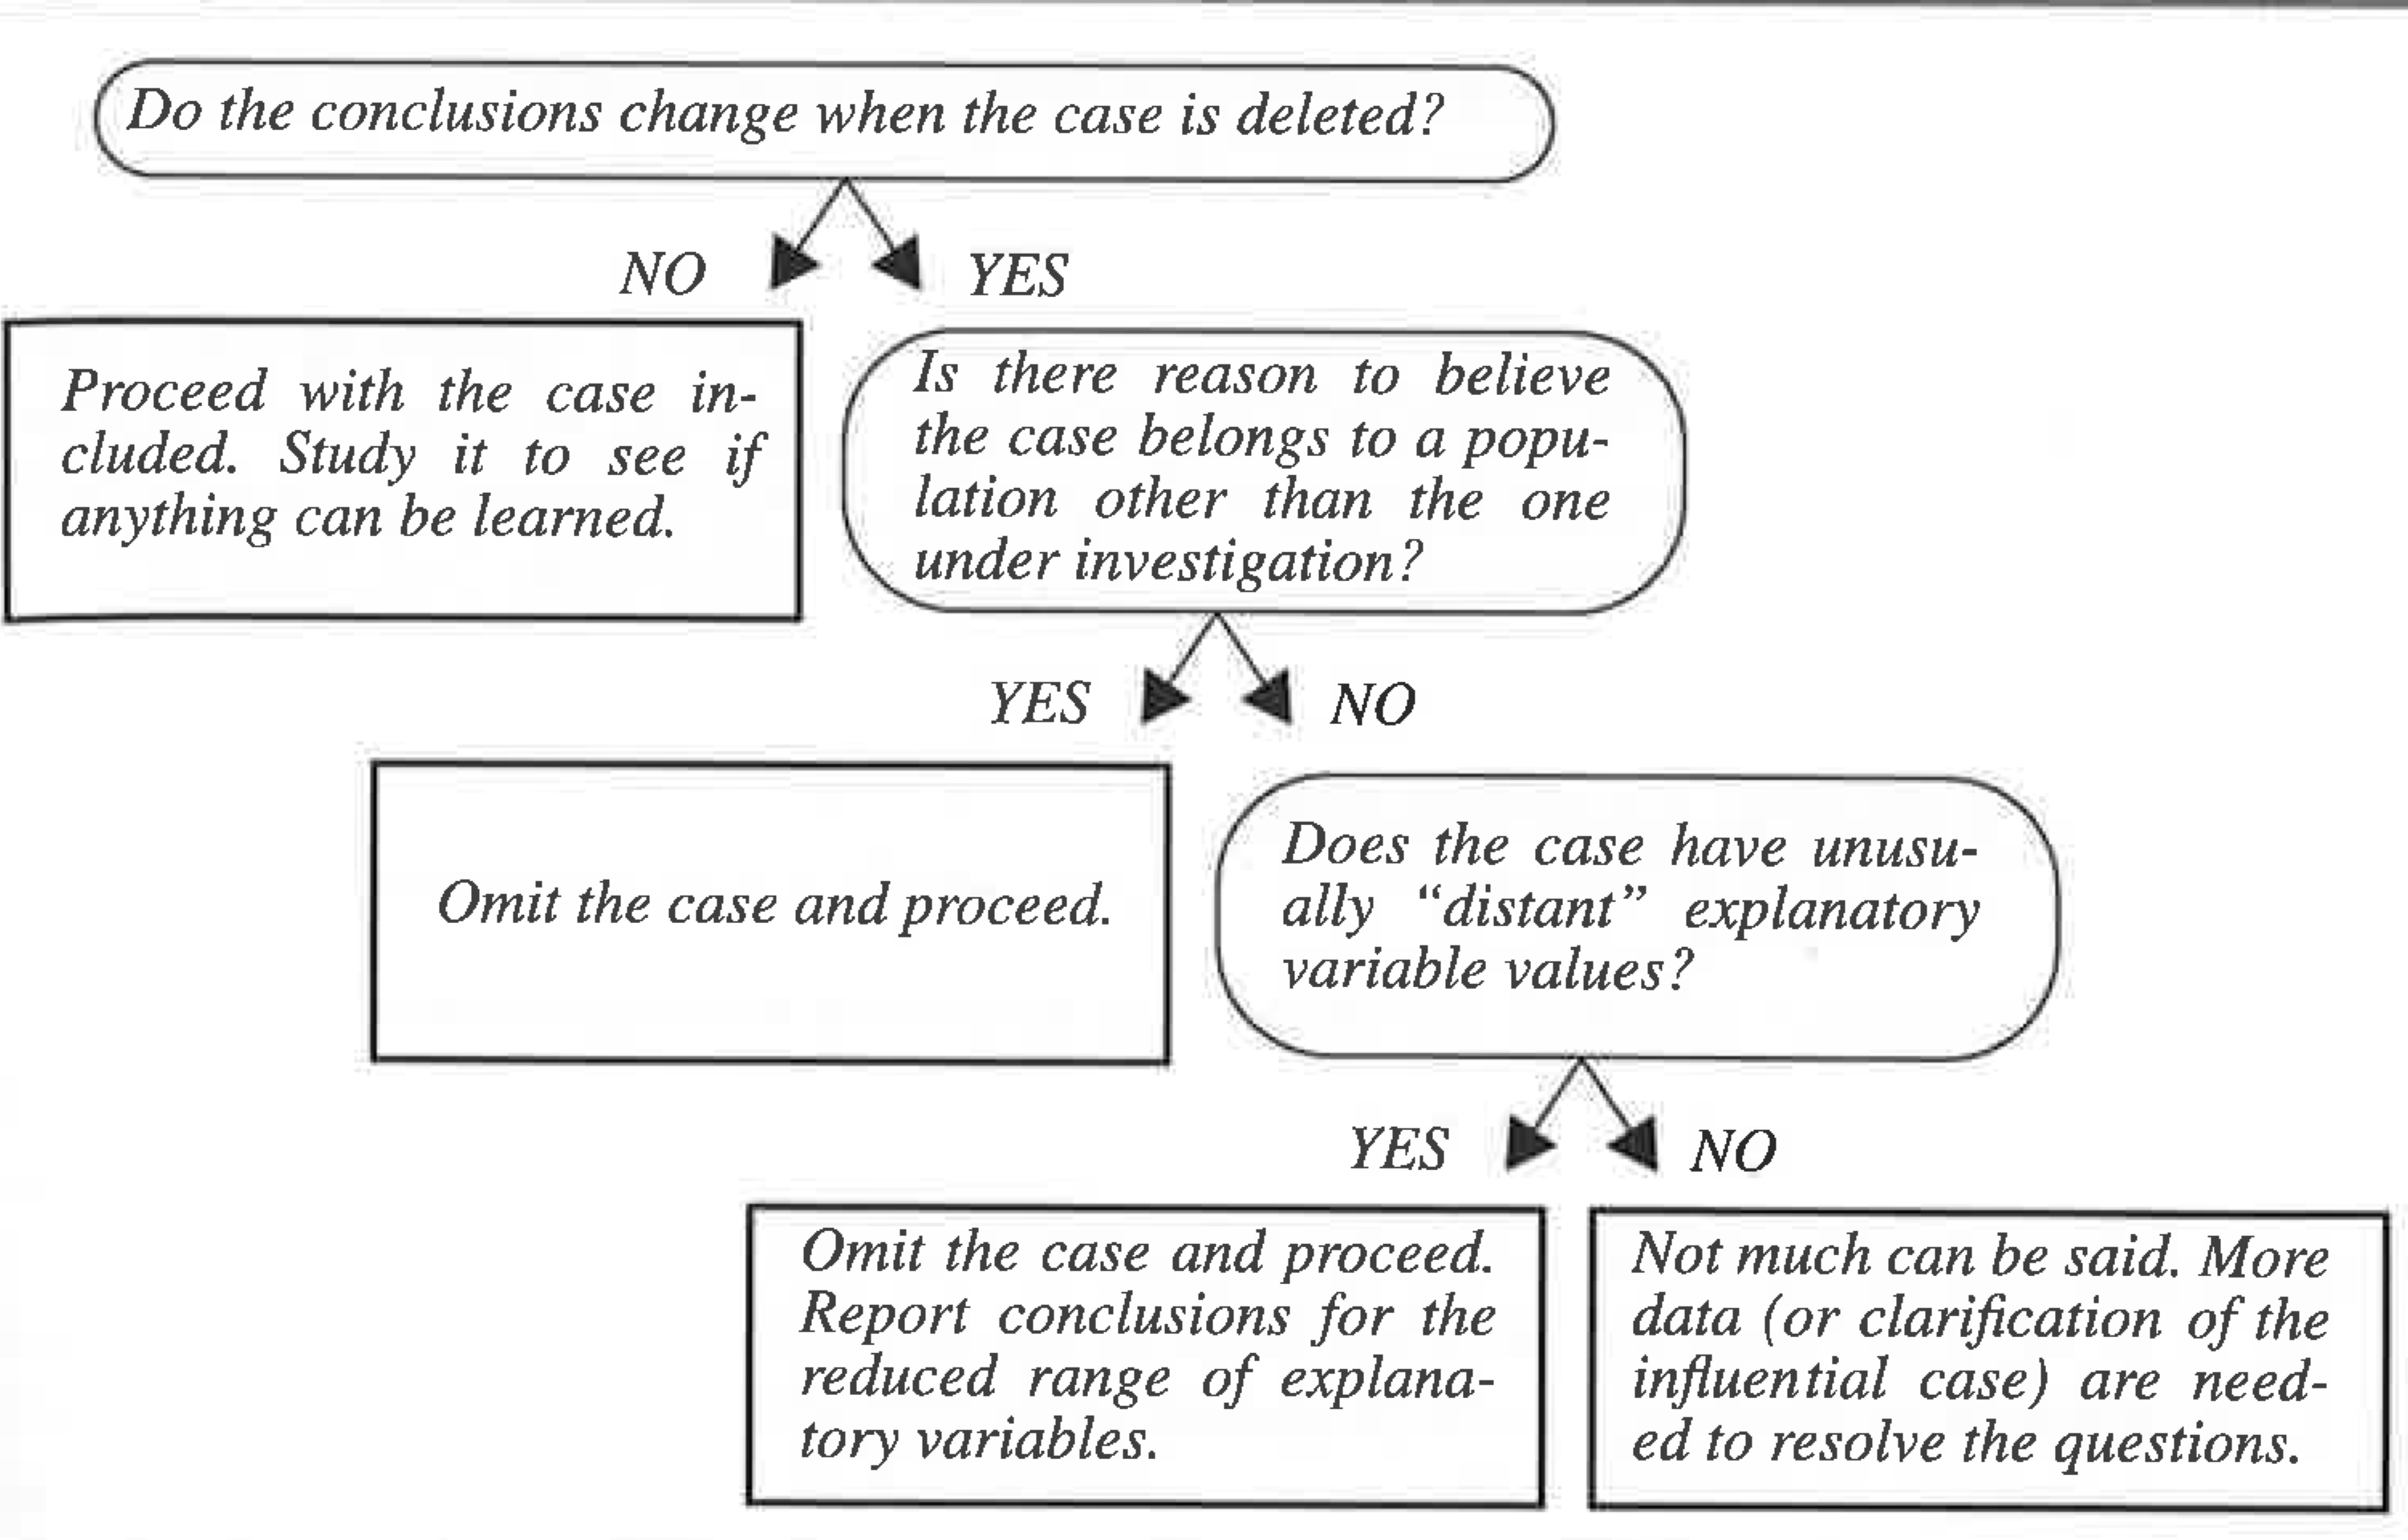
\includegraphics[width=0.8\textwidth,height=\textheight]{img/sleuth_outlier_flowchart.png}



\end{document}
